\documentclass[a4paper,12pt]{report}
\usepackage[slovene]{babel}
\usepackage{listings}
\usepackage{graphicx}
\usepackage[section]{placeins}
\graphicspath{ {./pics/} }
\newcommand{\subtitle}[1]{%
  \posttitle{%
    \par\end{center}
    \begin{center}\large#1\end{center}
    \vskip0.5em}%
}

\lstset{
numberstyle=\small, 
numbersep=8pt, 
frame = single, 
language=SQL, 
framexleftmargin=15pt}

\begin{document}

\title{Skripta za pripravo na ustni izpit:\\Planiranje in upravljanje informatike}
\author{Jakob Marušič}

\maketitle

\chapter{Uvodni sklop}

\paragraph{Informacijska družba} je družba v kateri je uspeh posameznika in organizacije 
odvisen od hitrosti procesiranja informacij in sposobnosti pridobiti pravo informacijo v pravem trenutku.

Informatiko moramo tretirat kot poslovno kategorijo (ne kot tehnologijo) ter kot investicijo (ne kot strošek).

\section{Obvadovanje informatike v splošnem}

\paragraph{Obvladovanje organizacije} je zagotavljanje struktur (organizacije in poslovanja) za določanje ciljev in nadzornih mehanizmov, ki zagotavljajo doseganje teh ciljev. Obvladovanje opredeljuje:
   \begin{itemize}
      \item organizacijsko strukturo,
      \item pravila in odgovornost za spremljanje odločitev na določenem področju,
      \item prosece
   \end{itemize}

Obvladovanje informatike je analogno obvladovanju drugih področji - na primer finančni direktor vzpostavi strukturo in pravila poslovanja za ogvoronost podpisovanja računov. Sam pa definira in spremlja matrike porabe sredstev.

\paragraph{Definicija} Obvladovanje informatike so vodstvene in ostale strukture ter procesi, ki omogočajo vzpostavitev takšne informatike v podjetju, ki bo omogočila izpolnitev in doseganje strategije podjetja.

Učinkovito obvladovanje naslavlja 3 vprašanja:
\begin{enumerate}
   \item Katere odločitve morajo biti sprejete, da bo zagotovljena učinkovita uporaba in upravljanje IT?
   \item Kdo sprejema te odločitve?
   \item Kako bo potekala realizacija in nadzor teh odločitev?
\end{enumerate}

\section{Obvladovanje informatike in poslovna strategija}

Obvladovanje informatike izhaja iz (poslovne) strategije poslovnega sistema z namenom učinkovite podpore poslovnim procesom in povečevanja uspešnosti poslovanja ter konkurenčnosti poslovnega sistema.
\textbf{Brez (dobre) poslovne strategije ni možno zasnovati (dobre) strategije informatike.}

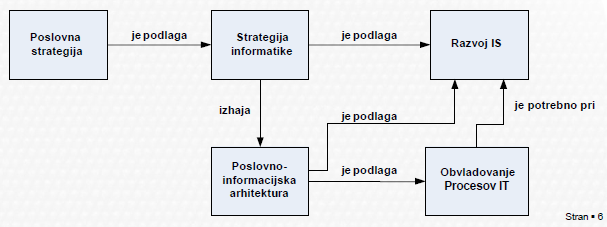
\includegraphics[scale=0.75]{001.png}

\section{Koncepti obvladovanja informatike}

\paragraph{Področja odločanja} v okviru obvladovanja informatike:
\begin{itemize}
   \item \textbf{Principi}: opredelitev poslovne vloge informatike
   \item \textbf{Arhitektura}: opredelitev standarizacije in potrebe po integraciji
   \item \textbf{Infrastruktura}: opredelitev potrebnih tehnoloških resursov in storitev
   \item \textbf{Poslovne aplikacije}: opredelitev potrebe po poslovnih aplikacijah (lahko so razvite interno, s strani zunanjih izvajalcev ali pa gre za redne produkte na trgu)
   \item \textbf{Investicije in prioritete}: izbor projektov za izvedbo in njihove prioritete
\end{itemize}

\paragraph{Nosilci odločanja} so lahko različni, od tega je odvisen način odločanja:

\begin{center}
   \begin{tabular}{||l|l||}
      \hline
      \textbf{Odločevalec} & \textbf{Način odločanja} \\
      \hline
      Vodstvo & poslovna monarhija \\
      Informatiki & IT monarhija \\
      Vsaka enota zase & fevdalizem \\
      Vodstvo in vodje enot & federalizem \\
      Informatiki in vodstvo & IT dualizem \\
      Posamezniki ali neformalne skupine & anarhija \\
      \hline
   \end{tabular}
\end{center}

\section{Karakteristike dobrega obvladovanja informatike}

\paragraph{Razumevanje obvladovanja in postopkov obvladovanja} učinkovitost obvladovanja informatike v podjetju je premosorazmerna z številom vodstvenega kadra, ki zna pojasniti postopke obvladovanja.

\paragraph{Način komunikacije na področju obvladovanja} ali so v podjetju formalna telesa in organi za obvladovanje informatike, ali obstaja pisarna za obvladovanje informatike ali Pisarna CIO

\paragraph{Stopnja direktne vključenosti vodstva} učinkovitost in kvaliteta obvladovanja se poveča s število vključenih CxO v obvladovanje informatike

\paragraph{Jasnost poslovnih cilje za investicije v informatiko}, npr. zmanjšanje stroškov, izboljšanje komunikacije, izboljšanje kvalitete,\dots

\paragraph{Stopnja odobrenih odstopanj} glede na interne standarde, zaradi hitrih spremeb je "zdravo", da se odstopanja odobravajo.

\paragraph{Stopnja sprememb v strukturi} in postopkih obvladovanja - učinkovito okolje je dolgotrajen proces.

\chapter{Obvladovanje IT po COBITu}

\paragraph{Definicija} Obvladovanje IT je struktura razmerij in procesov za usmerjanje in nadzor podjetja z namenom doseganja ciljev podjetja z dodajanje vrednosti, pri čemer uravnoveša tveganje ter korist IT in njenih procesov.

\paragraph{Zakaj potrebujemo standard?} Standar institucionalizira dobre prakse za zagotovitev, da IT podjetja podpira poslovne cilje.

\section{COBIT usmeritve}

\paragraph{Poslovna usmeritev} COBIT-a predstavlja:
\begin{itemize}
   \item povezovanje poslovnih in IT ciljev
   \item zagotavljanje metrik in modelov za merjenje doseganja
   \item opredelitev povezanih odgovornosti lastnikov poslovnih in IT procesov
\end{itemize}

\paragraph{Procesna usmeritev} je prikazana s procesnim modelom, ki IT ločuje na štiri domene in 34 procesov.

\paragraph{Koncepti arhitekture podjetja} pomagajo prepoznati bistvene vire za uspešnost poslovnih procesov - aplikacije, informacije, Infrastrukturo in ljudi.

\subsection{Logične skupine IT procesov}
\begin{enumerate}
   \item PO (Plan and Organize) - načrtovanje in organizacija
   \item AI (Acquire and Implement) - nabava in vpeljava
   \item DS (Delivery and Support) - izvajanje in podpora
   \item ME (Monitor and Evaluate) - spremljanje in vrednotenje
\end{enumerate}

\section{COBIT kot orodje}

\subsection{Delitev na ravni glede na namen}
\begin{enumerate}
   \item vodstvu in upravam
   \item poslovnemu vodstvu in vodstvu 
   \item strokovnjakom za upravljanje in zagotavljanje jamstev, nadzor in varnost
\end{enumerate}

\subsection{Koristi vpeljave}
\begin{itemize}
   \item standarizacija vpogleda v delovanje IT
   \item jasno lastništvo in zadolžitve na podlagi procesne usmeritve
   \item medsebojno razumevanje udeležencev na podlagi skupnega jezika
\end{itemize}

\subsection{Poslanstvo ogrodja}

Raziskovati, razvijati, objavljati in spodbujati avtoritativen, sodoben in
mednarodno sprejet okvir za obvladovanje IT, ki ga lahko sprejmejo
podjetja in je namenjen vsakodnevni uporabi s strani vodilnih v podjetju,
strokovnjakov s področja IT in strokovnjakov za zagotavljanje jamstev.

\subsection{Osredotočenost na poslovanje}
   COBIT po obliki ni namenje zgolj izvajalcem storitev IT, temveč posredno ali neposredno zagotavlja navodila vodstvu in lastnikom poslovnih procesov.

\subsection{Usmerjenost na procese}
   COBIT opredeljuje dejavnosti IT v okviru splošnega procesnega modela znotraj štirih domen. Te domene so:
   \begin{itemize}
      \item PO (Plan and Organize) - načrtovanje in organizacija
      \item AI (Acquire and Implement) - nabava in vpeljava
      \item DS (Delivery and Support) - izvajanje in podpora
      \item ME (Monitor and Evaluate) - spremljanje in vrednotenje
   \end{itemize}

\subsection{Kontrole}
   COBIT opredeli kontrolne cilje na vseh 34 procesih. Kontrola je opredeljena kot politika, postopek, praksa ali organizacijska struktua oblikovana za zagotavljanje razumnega jamstva, da bodo poslovni cilji doseženi.

\subsection{Vodenje z meritvami}
   Osnovna potreba vsakega podjetja je zagotoviti razumevanje stanja lastnih sistemov in se odločiti, kakšno raven upravljanja in kontrole zagotoviti. COBIT zagotavlja zrelostne modele za primerjalno analizo in prepoznavanje potrebnih izboljšav.

\section{IT procesi ogrodja COBIT}
   \subsection{Domena PO - načrtovanje in organizacija}
      \begin{center}
         \begin{tabular}{|l|l|}
            \hline
            \textbf{Oznaka procesa} & \textbf{Ime procesa} \\
            \hline
            PO1 & Opredelitev strateškega načrta za IT \\
            PO2 & Opredelitev informacijske strukture \\
            PO3 & Določitev tehnološke usmeritve \\
            PO4 & Opredelitev procesov, organizacije in razmerja IT \\
            PO5 & Upravljanje investicij v IT \\
            PO6 & Sporočanje ciljev in usmeritev vodstva \\
            PO7 & Upravljanje človeških virov v sektorju IT \\
            PO8 & Upravljanje kakovosti \\
            PO9 & Ocenjevanje in obvladovanje tveganj IT \\
            PO10 & Upravljanje projektov \\
            \hline
         \end{tabular}
      \end{center}

      \subsection{Domena DS - izvajanje in podpora}
      \begin{center}
         \begin{tabular}{|l|l|}
            \hline
            \textbf{Oznaka procesa} & \textbf{Ime procesa} \\
            \hline
            DS1 & Opredelitev in upravljanje ravni storitve \\
            DS2 & Upravljanje storitev tretjih strank \\
            DS3 & Upravljanje delovanja in zmogljivosti \\
            DS4 & Zagotovite neprekinjenost storitev \\
            DS5 & Zagotovite varnost sistemov \\
            DS6 & Ugotovite in porazdelite stroške \\
            DS7 & Izobrazite in usposobite uporabnike \\
            DS8 & Upravljajte službo za pomoč uporabnikom in obvladujte incidente \\
            DS9 & Upravljajte konfiguracijo \\
            DS10 & Ipravljanje problemov \\
            DS11 & Upravljanje podatkov \\
            DS12 & Upravljanje fizičnega okolja \\
            DS13 & Upravljanje delovanja \\
            \hline
         \end{tabular}
      \end{center}

      \subsection{Domena AI - nabava in vpeljava}
      \begin{center}
         \begin{tabular}{|l|l|}
            \hline
            \textbf{Oznaka procesa} & \textbf{Ime procesa} \\
            \hline
            AI1 & Določite avtomatizirane rešitve (aplikacije) \\
            AI2 & Nabavite in vzdržujte aplikacijske programe \\
            AI3 & Nabavite in vzdržujte tehnološko infrastrukturo \\
            AI4 & Omogočite delovanje in uporabo \\
            AI5 & Zagotovite vire IT \\
            AI6 & Upravljajte spremembe \\
            AI7 & Namestite in potrdite rešitve in spremembe \\
            \hline
         \end{tabular}
      \end{center}

      \subsection{Domena ME - spremljanje in vrednotenje}
      \begin{center}
         \begin{tabular}{|l|l|}
            \hline
            \textbf{Oznaka procesa} & \textbf{Ime procesa} \\
            \hline
            ME1 & Spremljajte in vrednotite delovanje IT\\
            ME2 & Spremljajte in vrednotite notranje kontrole\\
            ME3 & Zagotovite skladnost z zunanjimi zahtevami\\
            ME4 & Zagotovite upravljanje IT\\
            \hline
         \end{tabular}
      \end{center}

\chapter{Zunanje izvajanje}
      Vsaka aktivnost, naloga, delo ali proces, ki bi ga lahko izvedli zaposleni v delovnem času, ampak ga izvaja zunanji izvajalec za daljši čas.

      \paragraph{Prednosti}
      \begin{itemize}
         \item usmeritev na glavno dejavnost podjetja
         \item zmanjšanje stroškov
         \item transparentnost stroškov
         \item višji nivo storitev
         \item merljivost izvajanja storitev
         \item plačilo glede na opravljeno storitev
         \item zmanjšanje tveganja
         \item dostop do novih znanj in rešitev
         \item visoka varnost in zanesljivost
         \item hitrejše prilagajanje novim razmeram
      \end{itemize}

      \paragraph{Slabosti}
         \begin{itemize}
            \item izguba ključnih zmožnosti
            \item izguba nadzora
            \item odvisnost od zmožnosti drugega podjetja
            \item zmanjšanje možnosti sodelovanja med oddelki
         \end{itemize}

      \section{Tipični primeri zunanjega izvajanja}
         \begin{itemize}
            \item storitve podatkovnega centra
            \item storitve centra za pomoč uporabnikom
            \item varnostne storitve
            \item implementacija standariziranih rešitev
            \item aplikacije kot razvoj po naročilu (razvoj, tetiranje, vzdrževanje)
         \end{itemize}

      \section{Računalništvo v oblaku}
         \paragraph{Definicija (NIST)} Računalništvo v oblaku je model, ki omogoča priroče, povsod dosegljiv dostop do omrežja na zahtevo za skupni nabor nastavljivih računalniških virov.

         \subsection{Modeli storitev računalništva v oblaku}
            \paragraph{Programska oprema kot storitev (SaaS)} je aplikacija, ki se izvaja na ponudnikovi infrastrukturi katere pa se uporbanik ne zaveda. Uporabnik ima omejene možnosti konfiguracije.

            \paragraph{Platforma kot storitev (PaaS)} ponudnik zagotavlja in kontrolira okolje, v katerem uporabnik razvije svoje aplikacije. Uporabnik ima kontrolo nad svojimi aplikacijami in lahko delno konfigurira okolje.

            \paragraph{Infrastruktura kot storitev (IaaS)} ponudnik uporabniku omogoči zgolj osnovno infrasturkturo (procesor, omrežje, pomnilnik, \dots)

         \subsection{Finančna analiza}
            Inicialni strošek najema je nizek ali pa ga sploh ni. Vendar se na dolgi rok (več kot 5 let) lahko izkaže, da je pri najemu enakih kapacitet najem dražji od lastništva.

      \section{Kompetence ponudnikov zunanjega izvajanja}
         \paragraph{Kompetence dobave storitev} kako dobro se zmore dobavitelj odzvati na dnevne zahteve stranke z vidika stroškov, kakovosti, robustnosti in fleksibilnosti storitev.

         \paragraph{Kompetence transformacije} kako dobro se zmore dobavitelj storitve izboljšati glede funkcionalnosti, stroškov in kakovosti storitve.

         \paragraph{Kompetence odnosa} do katere mere je ponudnik storitev pripravljen na \emph{"win-win"} odnos.
      
      \section{Pogodbe s ponudniki storitev}
         \paragraph{Service leve agreement - SLA} mora vsebovati skupni dogovor o storitvah, prednostnih nalogah, odgovornostih, jamstvih in garancijah.
         \paragraph{SLA pokriva}
            \begin{itemize}
               \item seznam storitev, ki jih zunanji izvajalec pokriva
               \item naloge in odgovornosti pogodbenih strank
               \item ceno
               \item sledenje in poročanje
               \item ravnanje v primeru težav
               \item NDA
               \item varnost in zasebnost
               \item prenehanje pogodbe
            \end{itemize}
         \paragraph{Koristno, da pokriva}
            \begin{itemize}
               \item možnost nadzora
               \item pravico do odstopa do pogodbe
               \item pogodbene kazni
            \end{itemize}


\chapter{Strateško planiranje}
   \paragraph{Strateško planiranje v splošnem} Obsatajata dve vrsti managmenta - strateški in operativni. Prvi pridobiva napomenu šele v zadnjem obdobju, delimo ga na intuitivno strateško planiranje in formalno strateško planiranje.

   \section{Ključni procesi managmenta}
         \begin{enumerate}
            \item Opredelitev splošnih ciljev
            \item Strateško planiranje - zasnova, izdelava in spremljanje izvajanja strategije
            \item Postavitev merljivih ciljev
            \item Opredelitev filozofije podjetja - vrednote, odnos, nenapisana pravila
            \item Planiranje organizacijske strukture
            \item Planiranje in uvajanje poslovnih procesov ter sprememb
            \item Zagotavljanje osebja
            \item Zagotavljanje opreme in pogojev dela
            \item Zagotavljanje kapitala in finančnih sredstev
            \item Postavljanje standardov
            \item Določanje programov in operativnih planov
            \item Zagotavljanje možnosti spremljanja izvajanja strategij, merljivih ciljev, procesov in programov
            \item Motiviranje in spodbujanje osebja za kvalitetno in učinkovito delo
         \end{enumerate}

   \section{Definicija strateškega planiranja}
      Splošnega ogrodja/sistem strateškega planiranja, ki bi ga lahko privzela vsaka organizacija ni. Strateško planiranje mora biti prilagojeno potrebam, specifikam in karakteristikam podjetja.
      
      \paragraph{Definicija streteškega planiranja (A)} Strateško planiranje je proces, ki opredeljuje strategijo podjetja in vse na to vezane odločitve.
      \paragraph{Definicija strateškega planiranja (B)} Strateško planiranje je formalna opredelitev smeri v katero bo šla organizacija.

      \subsection{Ostali pojmi}
         \paragraph{Poslanstvo (mission)} opredeljuje namen obstoja organizacije.
         \paragraph{Vizija (vision)} opredeljuje želeno bodoče stanje podjetja ali organizacije glede na njegovo poslanstvo in strateške usmeritve.
   
   \section{Karakteristike strateškega planiranja}
      \subsection{Usmerjenost v prihodnost}
         Sistematična identifikacija priložnosti in groženj za podjetje v prihodnosti omogoča lažje in kvalitetnejše odločanje v sedanjosti.

      \subsection{Procesna usmerjenost}
         Kontinuiran proces vnaprejšnje zasnove in izdelave strategije, ki določa kaj, kaj, kdo in kako z rezultati. Šele nato sledi izdelava podrobnih planov.

      \section{Filozofija}
         Način mišljenja in odnosa, ki mora stalno reagirati glede na predvidevanje prihodnosti. Vodstvo in ključni predsatvniki podjetja morajo verjeti, da je potrebno strateško planirati.

      \section{Struktura}
         Strateško planiranje povezuje več vrst planov: strateški, taktični letni in plan programov in projektov. Strateško planiranje mora obsegati sistematične in formalizirane napore podjetja, ki omogočajo doseganje ciljev in izvajanje strategije.

   \section{Kaj ne spada pod strateško planiranje?}
         \begin{itemize}
            \item sprejemanje odločitev za prihodnost \textbf{v naprej}
            \item planov, ki nastanejo v okviru strateškega planiranja, se ne držimo za vsako ceno
         \end{itemize}

   \section{Konceptualni in operativni model strateškega planiranja}
         \paragraph{Konceptualni model strateškega planiranja} predstavlja kako naj bi v vsebinskem smislu strateško planiranje \emph{izgledalo}
         \paragraph{Operativni model strateškega planiranja} predstavlja kako podjetje to izvaja. Operativni model je operacionalizacija konceptualnega modela.

         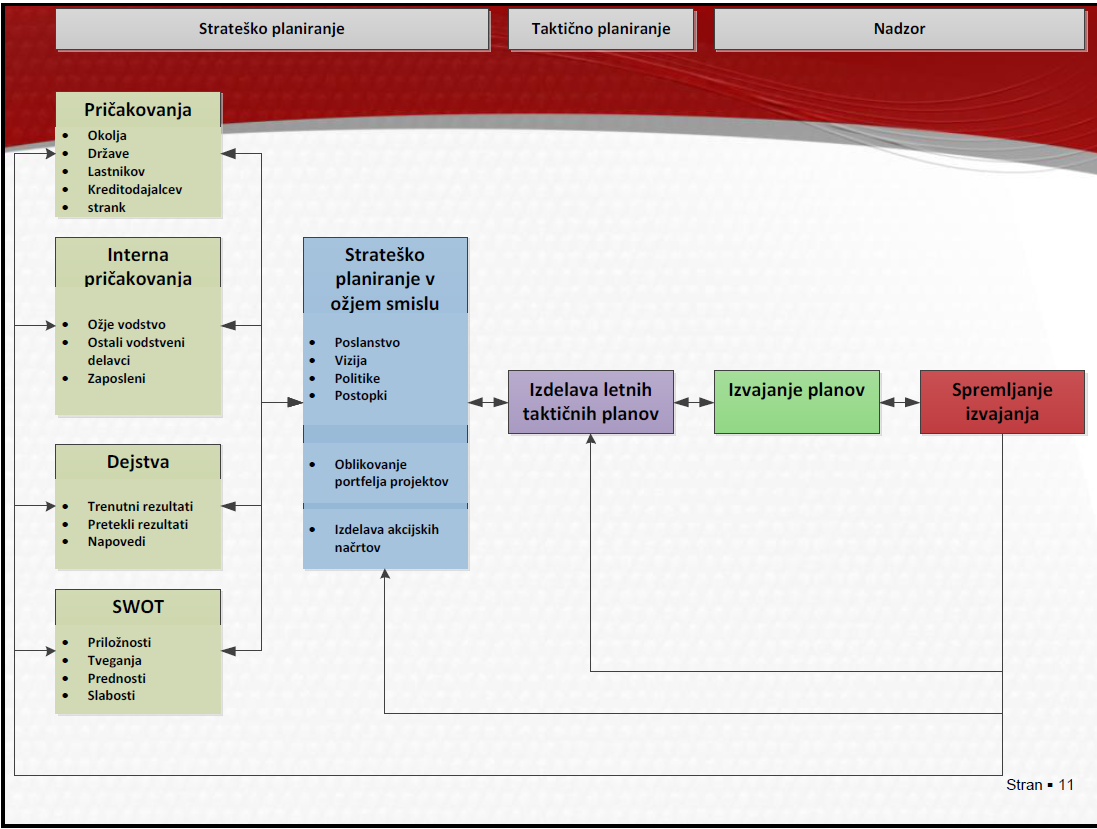
\includegraphics[scale=0.38]{002.png}
   
   \section{Načrt ukrepov ob nesrečah, načrt neprekinjenega delovanja}
      Strateški načrt temelji na najbolj verjetnih ocenah in predvidevanjih, \textbf{contingency plan} pa upošteva dogodke, ki so zelo malo verjetni, vendar lahko zelo vplivajo na podjetje. Contingency plan pomaga vodstvu soočiti se s situacijami, ki so malo verjetne in komaj predvidljive.

   \section{Stranski učinki strateškega planiranja}
      \begin{itemize}
         \item simuliranje prihodnosti
         \item uvajanje sistematičnih pristopov v podjetje
         \item uvajanje ciljne usmerjenosti
         \item uvajanje podlage za odločanje na vseh nivojih podjetja
         \item postavlja podlago za nadzor in spremljanje
         \item omogoča oz. postavlja podlago za merjenje učinkovitosti
         \item uvajanje mreže komuniciranja v podjetju
      \end{itemize}
   
   \section{Omejitve strateškega planiranja}
      \begin{itemize}
         \item nestabilno okolje
         \item interni odpor in ustaljene prakse
         \item planiranje ni poceni
         \item planiranje je zahteven proces
      \end{itemize}

   \section{Pristopi k planiranju}
      \paragraph{Top-Down} Plan izdela najvišje vodstvo v zelo centraliziranem podjetju ali pa poda vodstvo zgolj usmeritve oddelkom (če gre za necentralizirano podjetje).
      \paragraph{Bottom-Up} Vodstvo oddelkom ne izda usmeritev, zgolj zahtevo za oddajo planov.
      \paragraph{Kombinacija Top-Down in Bottom-Up} Ožje vodstvo poda grobe usmeritve, ki oddelkom omogočajo fleksibilnost pri izdelavi planov. Gre za najučinkovitejši način, ki spodbuja koordinacijo in planiranje med oddelki.
      \paragraph{Skupinsko planiranje} Je primerno za manjša podjetja. Ne primerno za podjetja, kjer je CEO avtoritativna oseba, ki ne prenapa kritik svojih idej in predlogov.

   \section{Napake pri strateškem planiranju}
      \subsection{Obdobje uvajanja}
         Gre predvsem za pomisleke za začetek uvajanja strateškega planiranja \emph{(npr. strateško planiranje ni potrebno, smo že poskusili vendar se ni obneslo,...)},
         pomisleke glede znanja v podjetju ter ne pripravljenost k spremebam.
      \subsection{Razumevanje filozofije in poslanstva}
         Ignoriranje dejstev strateškega planiranja, da gre za zahteven, a ne prezahteven proces. Ne razumevanje, da se je potrebno strateškemu planu prilagoditi tudi s starimi politikami in praksami, ki mogoče niso primerne.
      \subsection{Vpletenost najvišjega vodstva}
         Na eni strani gre za težavo premajhnega angažiranja vodstva v strateško planiranje (gre za planiranje za prihodnost, strateško planiranje ne rešuje sedanjih težav) in na drugi strani preveč centralizirano strateško planiranje (oddelki niso vključeni v planiranje).
      \subsection{Proces planiranja}
         Strateško planiranje ne sme vzpostaviti preveč togega in formalnega sistema, ki zavira fleksibilnost in kreativnost. Hkrati ne sme izdelati nerealnih planov in preveč podrobnih načrtov. Vseeno pa si je za izdelavo planov potrebno vzeti čas in jih v podjetju tudi skomunicirati.
      \subsection{Uporaba in izvajanje strateških planov}
         Sam strateški plan ni uporaben, če ga v podjetju ne izvajamo/uporabljamo. Pri sami uporabi pa si vseeno dovolimo fleksibilnost in kreativnost - strateškega plana se ne držimo kot pijanec plota.

\chapter{Strateško planiranje informatike}
   \paragraph{Definicija strateškega planiranja informatike} Strateško planiranje informatike je proces definiranja nabora aplikacij, ki so organizaciji v pomoč pri uresničevanju poslovnih planov in njenih poslovnih ciljev.
   Strateški plan informatike mora:
      \begin{itemize}
         \item izhajati iz poslovnega strateškega plana
         \item organizaciji omogočiti uresničitev strateških ciljev
         \item posredno zagotoviti konkurenčno prednost
      \end{itemize}

   \paragraph{Strateški plan digitalizacije} je \emph{bolj moderen} naziv za strateški plan informatike, ki se osredotoča na tehnologije digitalizacije:
      \begin{itemize}
         \item senzorje,
         \item avtonomne sisteme in naprave,
         \item digitalne dvojčke.
      \end{itemize}

   \paragraph{Strateško planiranje je kontinuiran proces} sestavljen iz procesov izdelave in uresničevanja, v katerem vodstveni delavci, notranji in zunanji strokovnjaki s področja informatike in uporabniki s partnerstvom tako pri izdelavi, uresničevanju in vrednotenju rezultatov zagotavljajo maksimalno izrabo informacijskih tehnologij za doseganje dolgoročne uspešnosti poslovnega sistema.

   \section{Izdelava strateškega plana in njegovo uresničevanje}
      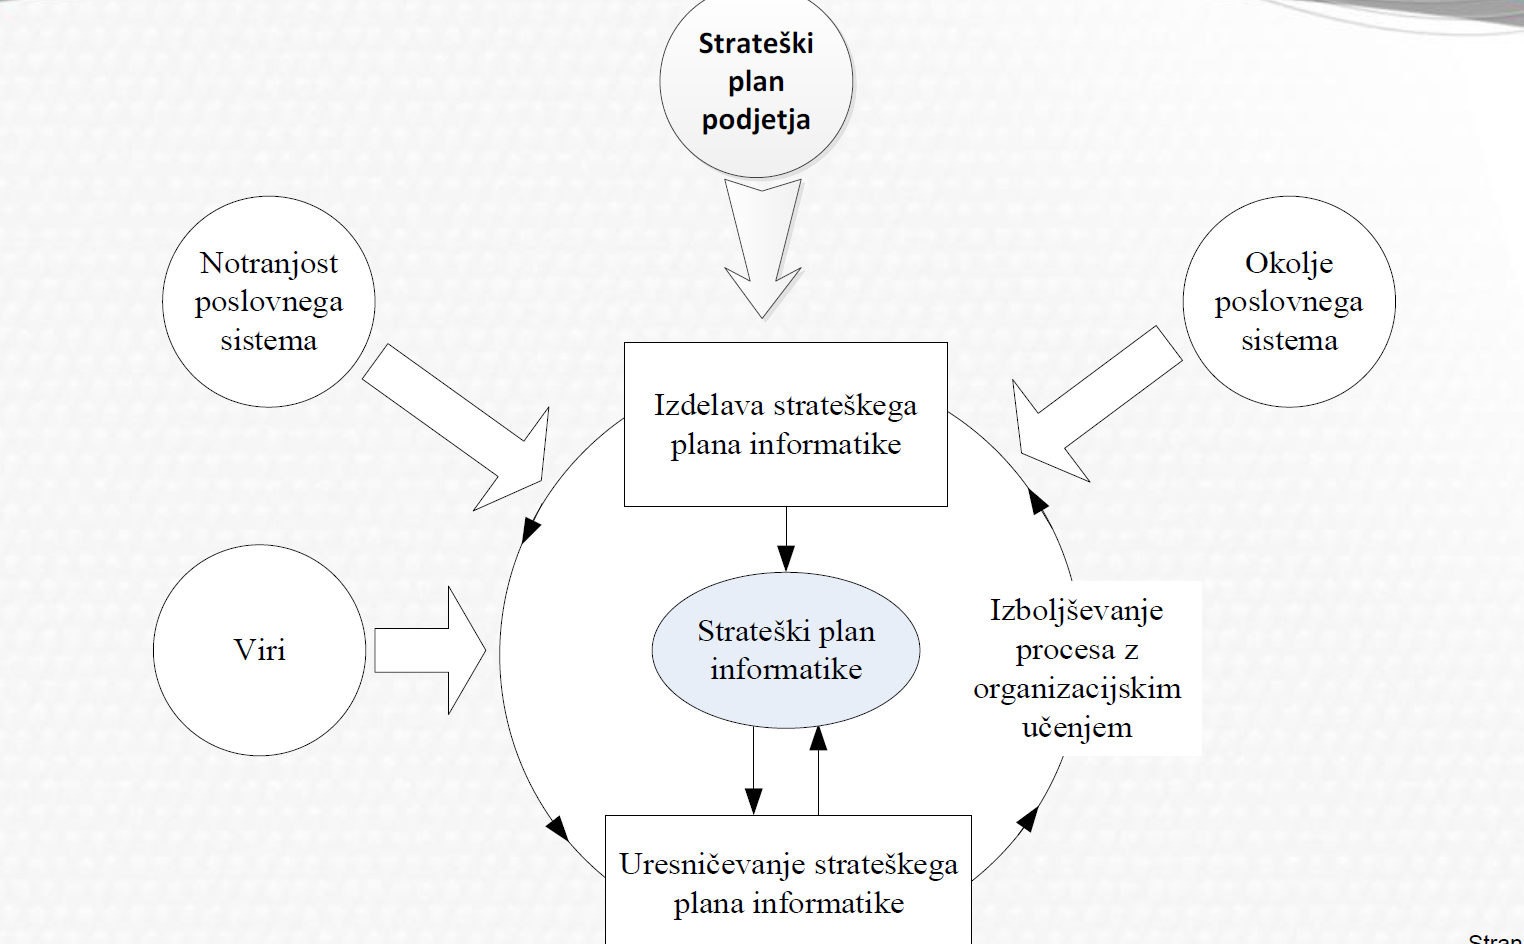
\includegraphics[scale=0.375]{003.png}

   \section{Poslovno informacijske arhitektura}
      \paragraph{Definicija} Poslovno-informacijska arhitektura je sistematični pristop k zajemanju in upravljanju:
         \begin{itemize}
            \item \textbf{poslovnih modelov}: modelov poslovnih procesov, organizacijske strukture, modelov funkcionalnih področji,\dots
            \item \textbf{modelov informacijske podpore}: aplikacije, integracije med aplikacijami v okviru informacijskega sistema,\dots
            \item \textbf{modelov tehnološke infrasturkture}
         \end{itemize}

      Obvladovati PIA pomeni poznavati delovanje poslovnih in odločitvenih procesov, nadzorovano uvajanje aplikacij (v smeri učinkovitosti in standarizacije) ter nadzorovano uvajanje konceptov, elemntov in tehnologij.

      PIA je primeren kot osnova za predstavitev in komuinikacijo, osnovo za načrtovanje in za zagotavljanje skladnosti in povezanosti vseh delov poslovnega sistema.

   \section{Metodologija strateškega planiranja informatike}
      \paragraph{Koncepti}
         \begin{itemize}
            \item vloge
            \item postopki \emph{(pregled in analiza stanja, opredelite obstoječe PIA, vizije IT, vizije PIA, projektov, spremljanje izvajanja)}
            \item aktivnosti
            \item izdelki
         \end{itemize}
      \paragraph{Teoretične osnove}
         \begin{itemize}
            \item tehnike
            \item pristopi
         \end{itemize}

      \subsection{Področja obravnave}
         Področja obravnave obsegajo informacijsko podporo procesom, odločanju in vodstvu, dokumentni sistem, elektronsko in mobilno poslovanje, skupno IT infrastrukturo, obvladovanje informatike,\dots
      
      \subsection{Strateški elementi}
         Strateški elementi obsegajo vizijo in poslantvo, poslovno strategijo (usmeritve, cilje in probleme), informacijski sistem (usmeritve, cilje in probleme) ter matrike (cilje IS in cilje PS ter cilje IS in probleme PS).

      \subsection{Model informacijskega sistema}
         Model informacijskega sistema prikazuje tako interne aplikacije ter povezave med njimi (\textbf{model notranje povezanosti}) kot tudi aplikacije in njihovo povezanost z zunanjimi sistemi (\textbf{model zunanje povezanosti}).
         \paragraph{Vizija} Vizija opredeljuje potrebne spremembe za vsa področja obravnave in željeno ciljno stanje. Vizija lahko povzroči problem prenove poslovnih sistemov in prilagajanje informacijske podpore.

      \subsection{Model informacijske podpore poslovnega sistema}
         Model informacijske podpore poslovnega sistema prikazuje poslovne procese in aplikacije, ki jih informacijsko podpirajo.

      \subsection{Portfelj projektov}
         V portfelj projektov vnašamo opise projektov, katerih lahko način in novo podrobnosti variira. Projekt je lahko organizacijskega, pripravljalnega ali implementacijskega tipa in zadeva področje podpore odločanja, področje poslovnega informacijskega sistema ali podjetju specifičnega področja.


\chapter{Projektno vodenje}
   \section{Definicija projekta}
      \paragraph{Projekt} je začasno vzpostavljena organizacijska struktura, katere cilj je izdelati enkraten, nek točno določen izdelek, storitev ali rezultat.
      \paragraph{Začasno vzpostavljena organizacijska struktura} ima začetek in konec. Konec nastopi ko so cilji izpolnjeni ali, ko postane jasno, da ciljev ni mogoče izpolniti ali cilji niso več relavantni. Začasna struktura ne pomeni, da je projekt kratek v časovnem smislu.
      \paragraph{Tipski projekt} Pojem izhaja iz gradbeništva (gradnja enake stavbe kot v predhodnem projektu je nov projekt). V IT bi tipski projekt lahko bil uvedba sistema za evidenco časa v novi stavbi.
      \subsection{Učinki projekta}
         \begin{itemize}
            \item učinki kot poslediaca uporabe izdelkov projekta
            \item stranski učinki, ki so lahko negativni
         \end{itemize}
      \subsection{Tipi IT projektov}
         \begin{itemize}
            \item organizacijski
            \item načrtovalni
            \item izvedbeni za programsko opremo
            \item izvedbeni za strojno opremo
         \end{itemize}
   \section{Portfelj in program}
         \paragraph{Porfelj} je skupina podportfeljev, programov in projektov, ki potekajo oz. morajo potekati medsebojno koordinirano, ker skupaj izpolnjujejo enega ali več strateških ciljev podjetja. Vsi projekti v portfelju niso nujno medsebojuno odvisni.
         \paragraph{Program} je skupina medsebojno povezanih in odvisnih projektov, ki so vodeni in koordinirani v okrilju programa v smeri pridobivanja pozitivnih učinkov, ki ob individualnem in izoliranem vodenju ne bi bili možni.

   \section{Projektno vodenje - projektni managment}
      \paragraph{Definicija} Projektno vodenje je uporaba znanj, izkušenj, orodij in tehnik v okviru projektnih aktivnosti, ki omogočajo izvajanje projekta in izpolnitev ciljev projekta.

      \paragraph{Znanja in procesi na področju projektnega vodenja} PMBoK opredeljuje področja znanja:
         \begin{itemize}
            \item obvladovanje obsega projekta
            \item obvladovanje časovnih parametrov in trajanja projekta
            \item obvladovanje stroškov projekta
            \item obvladovanje kakovosto na projektu
            \item obvladovanje človeških virov
            \item komunikacija na projektu
            \item obvladovanje tveganj
            \item obvladovanje deležnikov projekta
            \item obvladovanje oskrbovanja
            \item obvladovanje integracije projekta
         \end{itemize}
      PMBoK opredeljuje naslednje skupine procesov:
         \begin{itemize}
            \item procesi inicializacije
            \item procesi planiranja
            \item procesi izvajanja
            \item procesi nadzora in kontrole
            \item procesi zapiranja
         \end{itemize}

         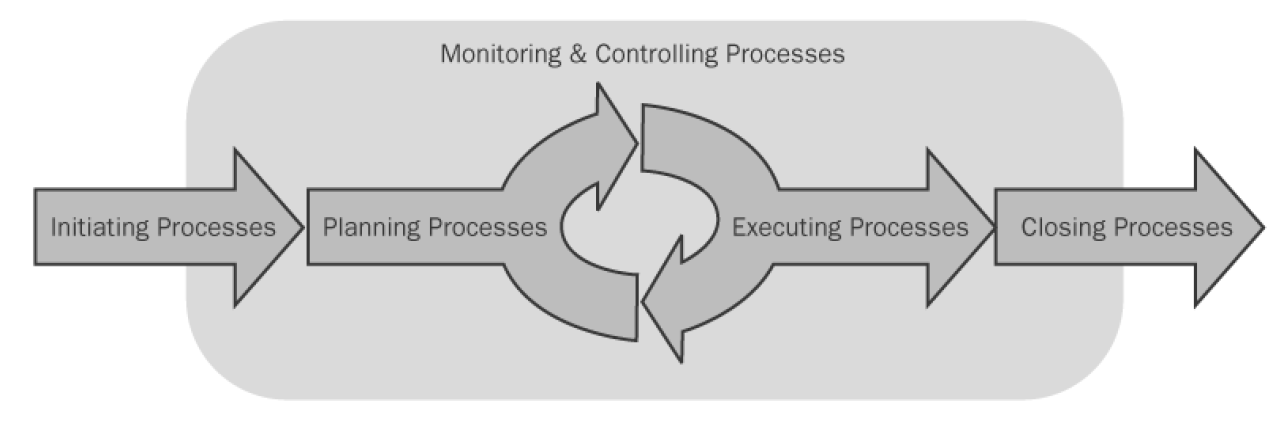
\includegraphics[scale=0.375]{004.png}

   \subsection{Vloge na projektu}
      \paragraph{Projektni vodja} (tudi vodja projekta): vodja projekta na strani naročnika in vodja projekta na strani (zunanjega) izvajalca
      \paragraph{Sponzor} je oseba, ki je direktno zainteresiran za uspeh projekta. Naročnik postane sponzor projekta, ko aktivno spremlja in podpira projekt (omogoči razbremenitev ključnih kadrov, zagotovi nove zaposlitve in dodatna sredstva,\dots).
      \paragraph{} Naročnik, uporabnik izdelka, član projektne ekipe, lastnik tveganja, prokurist, \dots
      \paragraph{Stakeholder - deležnik} Deležnik je vsaka oseba, na katero izdelki in učinki projekta posredno ali neposredno vplivajo. Deležnik je lahko projektu naklonjen ali ne ter ima od projekta določen interes. Deležniki so zelo različni: člani projektne ekipe, poslovodstvo, sponzorji, zunanji izvajalci, obstoječi dobavitelji, \dots

   \subsection{Organizacija projektne skupine}
      \paragraph{Matrična organizacija} Predstavlja konflikt med rednim delom in delom na projektu, za komunikacijo glede uskladitve obremenjenosti članov projektne ekipe je naloga vodje projekta.
         \begin{figure}[h]
            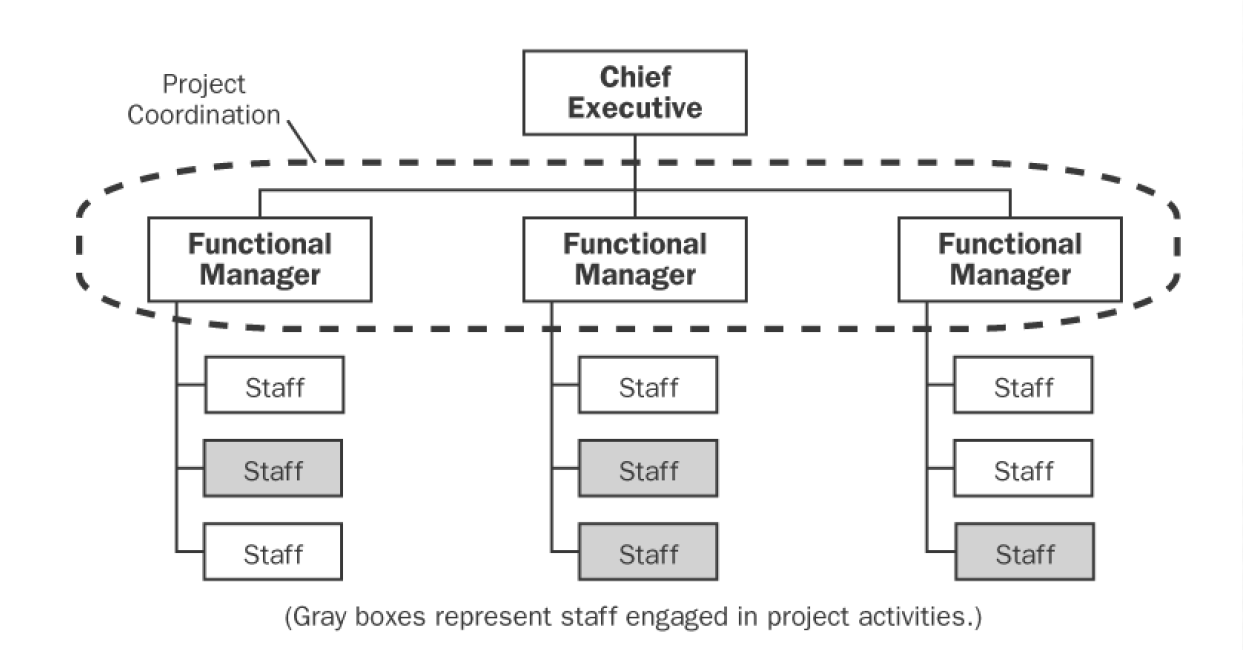
\includegraphics[scale=0.375]{005.png}
            \caption{Primer šibke matrične organizacije}
         \end{figure}
         \begin{figure}[h]
            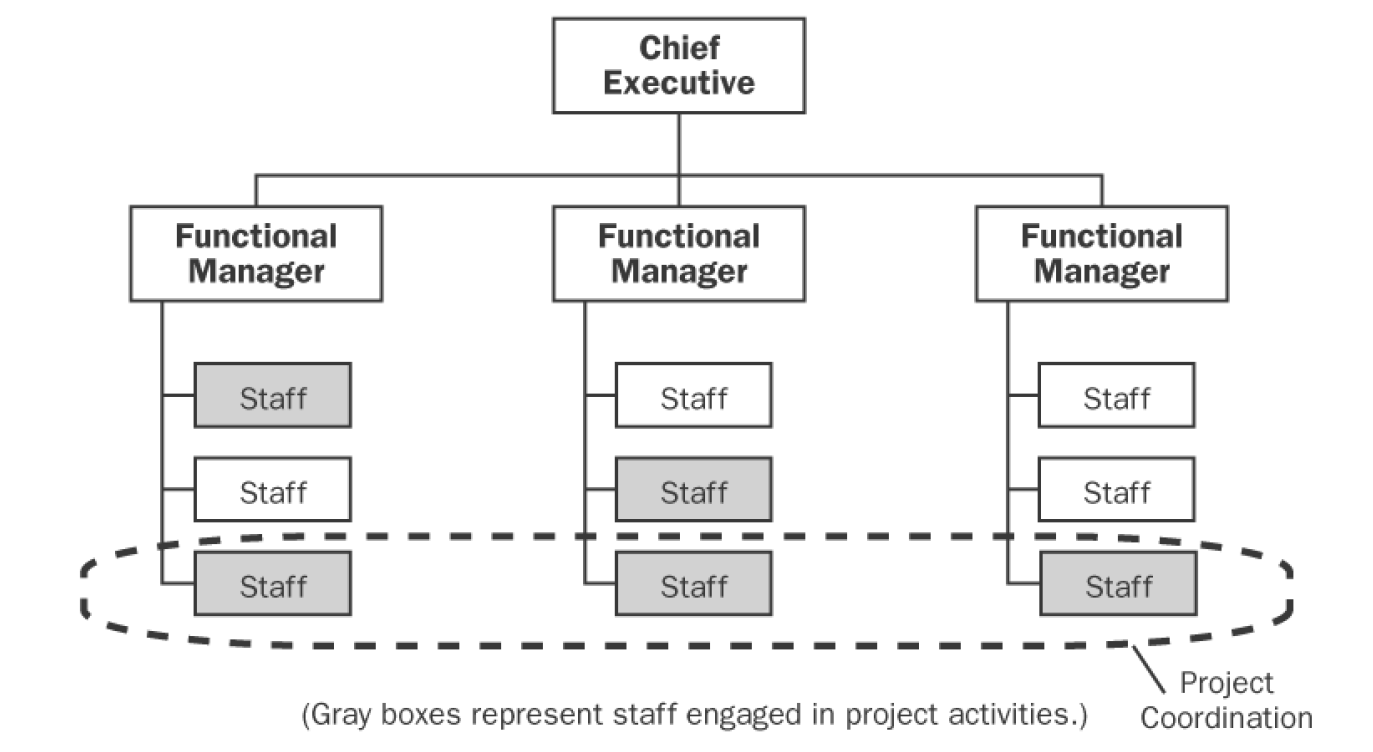
\includegraphics[scale=0.375]{006.png}
            \caption{Primer šibke matrične organizacije}
         \end{figure}
         \begin{figure}[h]
            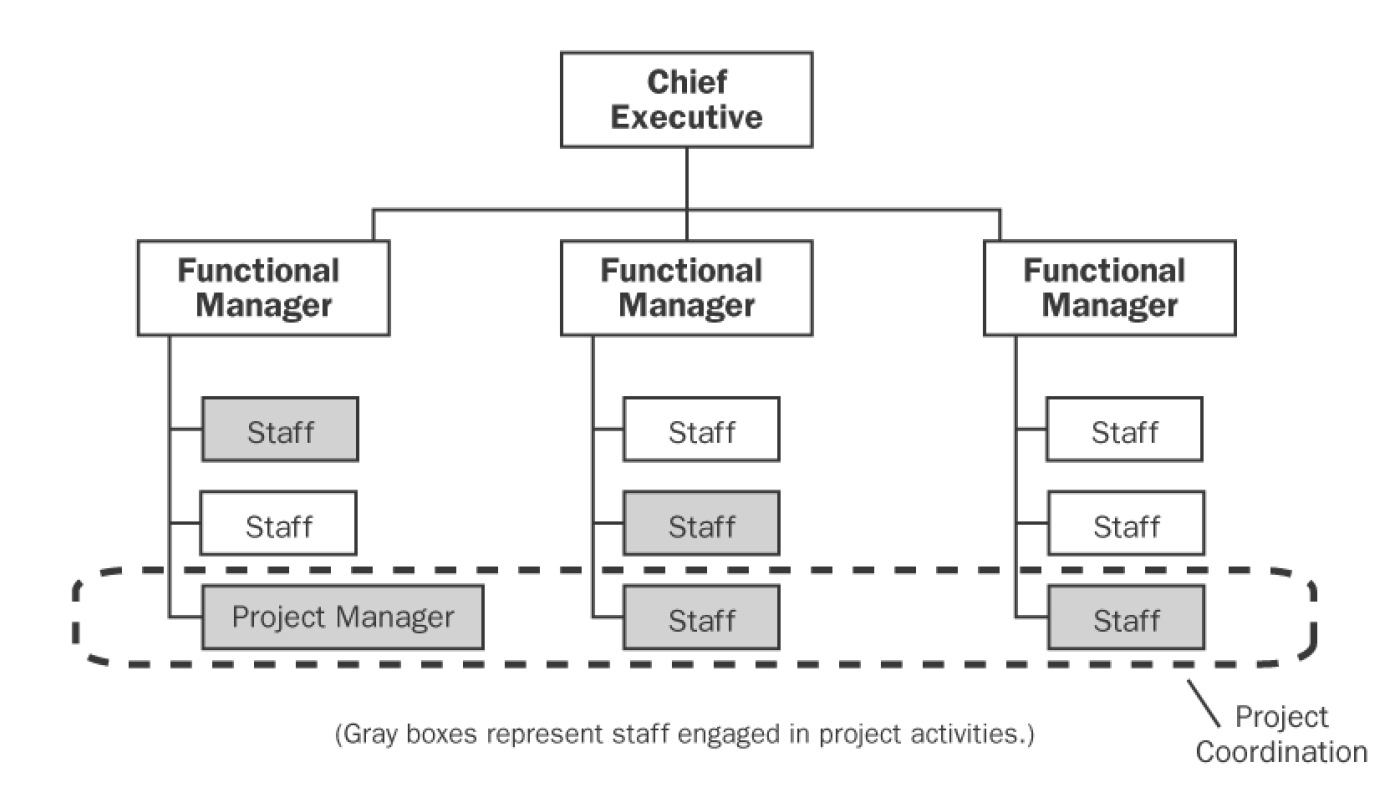
\includegraphics[scale=0.375]{007.png}
            \caption{Primer uravnotežene matrične organizacije}
         \end{figure}
         \begin{figure}[h]
            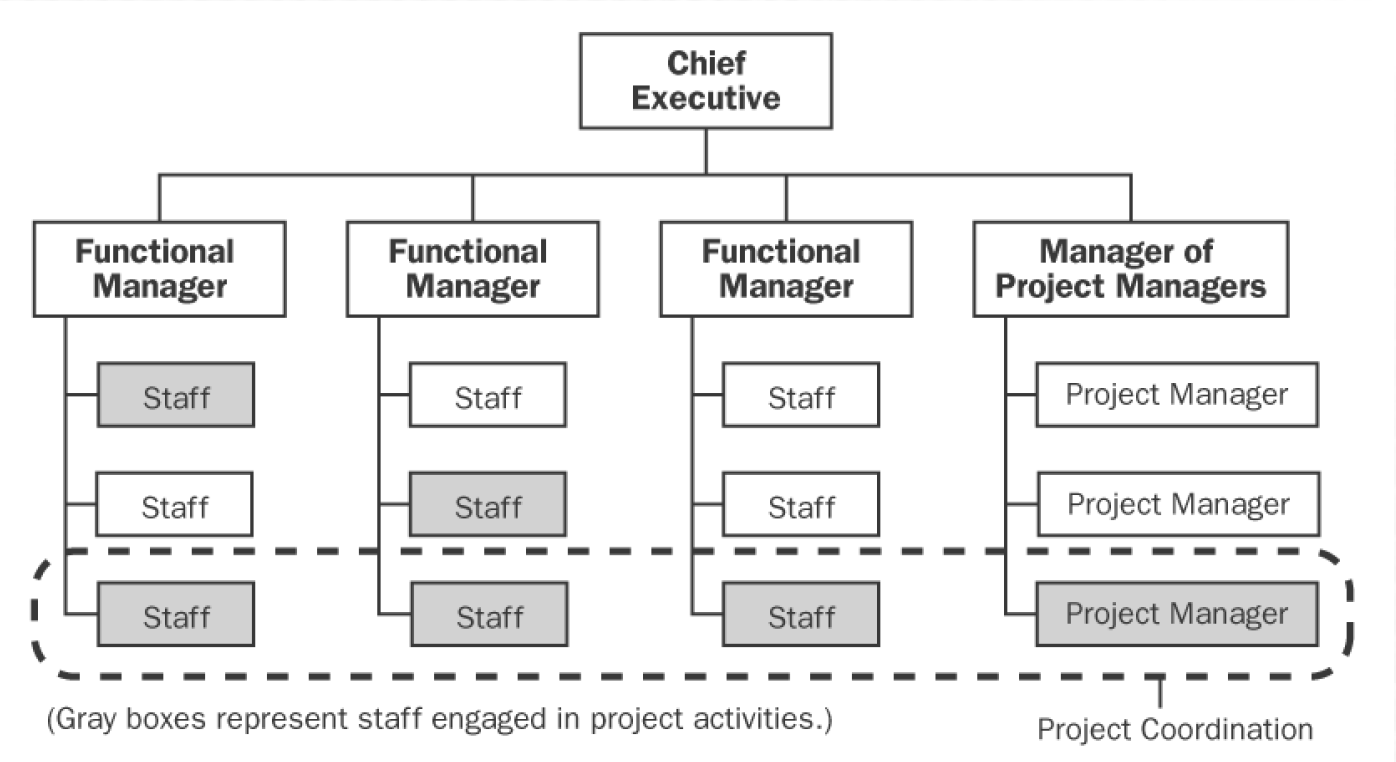
\includegraphics[scale=0.375]{009.png}
            \caption{Primer močne matrične organizacije}
         \end{figure}
         \begin{figure}[h]
            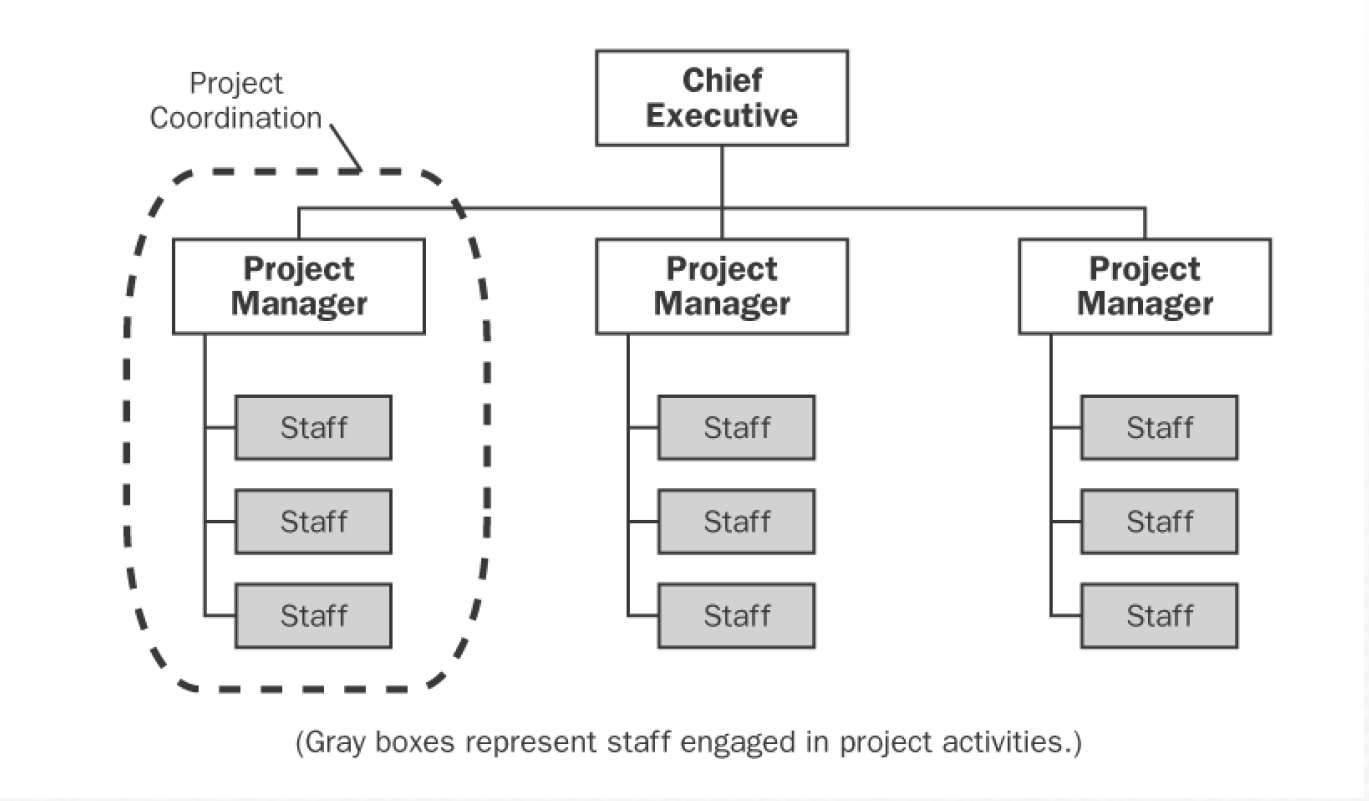
\includegraphics[scale=0.375]{008.png}
            \caption{Primer projektne organizacije}
         \end{figure}

   \section{Projektna pisarna}
         \paragraph{Projektna pisarna} Organizacijska enota za podporo projektom, ki niha med izvajanjem zgolj administrativnih nalog (arhiviranje in obvladovanje projektne dokumentacije, organizacija sestankov, zapisnikov,\dots) in strateško projektno pisarno (obvladovanje PMIS, izdelava podjetju primernih metodologij, vodenje portfeljev, programov in projektov, zagotavljenje izvajanja strategije podjetja,\dots).
   \section{Projektni svet}
      \paragraph{Projektni svet} je telo, ki v imenu naročnika spremlja in nadzoruje projekt s pristojnostmi potrjevanja, potrjevanja s pripombami, zavračanja mejnikov in izdelkov, potrjevanje ali zavračanjem zahtevkov po spremembi, zaustavljanjem projekta, potrjevanjem zaključka projekta, potrjevanjem VDP.
      \paragraph{Sestava projektnega sveta} Projektni svet je sestavljen iz vodstvenih kardov, izbranih poslovnih uporabnikov (ključni uporabniki), vodje projekta s strani naročnika.

   \section{Informacijska podpora projektom}
      \paragraph{Project Managment Information System (PMIS)} omogoča učinkovitejše vodenje in izvajanje projektov. Ključni mofuli PMIS so:
         \begin{itemize}
            \item dokumentni sistem
            \item koledarji
            \item obvladovanje WBS in gentograma
            \item spremljanje in nadziranje stroškov
         \end{itemize}
      \paragraph{} Razdeljevanje nalg, poročanje o izvedbi nalog in spremljanje izvajanja nalog je praviloma ločena aplikacija.

   \section{Tveganja na IT projektih}
      \subsection{Tipi tveganj}
         \paragraph{Splošna tveganja} Med njih štejemo belezni članov projektne ekipe, neustrezno sodelovanje, prebrnjenost članov ekipe, slabo podporo, (pre)kratki časovni roki, prekinitev financiranja.
         \paragraph{Tveganja s področja zakonodaje} Med potekom projekta se lahko zgodi sprememba zakonodaje, ki pokriva projekt ali pa zakonodaja sploh še ni sprejeta (bo srpejeta med potekom projekta).
         \paragraph{Tehnološlko-arhitekturan tveganja} so tveganja uporabe novih tehnologij (težava z integracijo, vprašljiva podpora,\dots), varnosti, migraciji podatkov iz starega v nov IS.
         \paragraph{Metodološka tveganja} se navezujejo na neopredeljenost project life cycle ali slabega razumevanja le tega s strani projektne ekipe.
         \paragraph{Tveganja vezana na končni izdelek} Uporabniki izdelka ne bodo sprejeli (se mu bodo uprli) ali pa člani projektne ekipe ne poznajo platforma na kateri izdelek bazira.
         \paragraph{Organizacijska tveganja} vključujejo možnost reorganizacije v podjetju med samim projektom ali pa zahteva po večji spremembi poslovnih procesov kot je bilo v začetku predvideno.
   \section{Statusna in zaključna poročila}
      \paragraph{Frekvenca statusnega poročila} naj bo določena v naprej (npr. enkrat na mesec), lahko pa je tudi na zahtevo.
      \paragraph{Namen statusnega poročila} Statusno poročilo projektnega vodjo prisili, da uredi in pretehta stanje na projektu.
      \paragraph{Prikrivanje} V poročilu ne smemo prikrivati stanja, kritičnih informacij, tveganj projekta.
   

\chapter{Projektno vodenje po PMBoK}
   \section{Inicializacija in zasnova projekta}
      \paragraph{VDP} Vzpostavitveni dokument projekta je najpogostejši izraz uporabljen v Sloveniji, po PMBoK standardu se uporablja izraz \textbf{projektna listina}. Ostali izrazi za VDP so projektni elaborat ali tehnični elaborat projekta.
      \subsection{Inputi inicializacije}
         V inicializaciji se moramo vprašati:
            \begin{itemize}
               \item Kaj so glavni cilji projekta?
               \item Kdo so deležniki?
               \item Kakšna je pozicija projekta v okviru portfelja (strategije) podjetja?
               \item Ali je v podjetju že bil \emph{enak} projekt in je bil neuspešen?
               \item Kakšna je \emph{klima} pri naročniku?
               \item Kultura v podjetju, ki je glavni nosilec in naročnik projekta
               \item Zakonski predpisi vezani na projekt
            \end{itemize}
      
      \subsection{Deležniki projekta}
         \paragraph{Proces identifikacije deležnikov projekta} V inicializaciji projekta je potrebno definirati deležnike projekta, ovrednotiti njihovo stanje (zanimanje in pričakovanja), vpliv in predvsem odnos do projekta (projekt lahko podpira ali mu nasprotuje).
         \paragraph{Obravnavanje nasprotnikov projekta} Obravnava nasprotnikov je predvsem pomembna, ko ima oseba velik vpliv na projekt oz. posredno na njegov rezultat. Ugotoviti je potrebno zakaj mu nasprotuje, razviti strategijo za komunikacijo z njim in razmisliti kako ga pridobiti na svojo stran.
            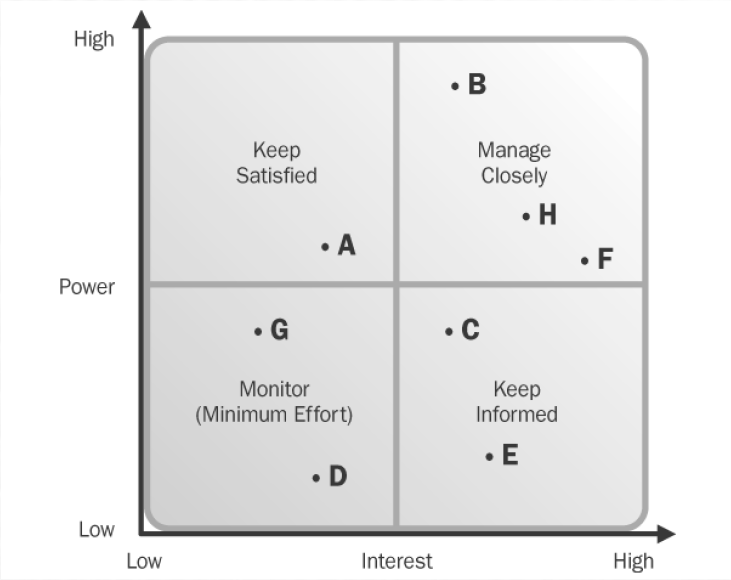
\includegraphics[scale=0.375]{010.png}

   \section{Obvladovanje obsega}
         \begin{center}
            \begin{tabular}{|l|l|}
               \hline
               \textbf{Proces področja obvladovanja obsega} & \textbf{Skupina procesov} \\
               \hline
               \hline
               Planiranje obvladovanja obsega & Procesi planiranja \\
               Zbiranje zahtev & \\
               Definiranje obsega & \\
               Izdelava WBS & \\
               \hline
               Overjanje obsega & Procesi nadzora in kontrole \\
               Kontroliranje obsega & \\
               \hline
            \end{tabular}
         \end{center}
      \subsection{Vsebinski pogled na obvladovanje obsega}
         \begin{center}
            \begin{tabular}{|l|l|}
               \hline
               \textbf{Vsebinski pogled} & \textbf{Proces} \\
               \hline
               Kaj potrebujemo? & Zbiranje zahtev \\
               Kaj moramo narediti? Katere izdelke? & Definiranje obsega \\
               Načrt tega, kar moramo narediti & WBS \\
               Ali naročnik meni, da gremo v pravo smer? & Veritificiranje obsega \\
               Interno obladujemo, da delamo to, kar je zahtevano & Kontroliranje obsega\\
               \hline
            \end{tabular}
         \end{center}
      \subsection{Izdelava WBS}
         \paragraph{WBS (Work Breakdown Structure)} Dekompozicijski diagram dela na večih nivojih razbije problem na manjše, obvladljive enote. Enota ni nujno manjši izdelek ali del izdelka. Lahko je karkoli, kar doprinese projektu (obvladovanje tveganj, kontrola kakovosti,\dots)
         \paragraph{Work Package} Delovni paket je največja enota WBS-a, ki ga realiziramo z eno ali več aktivnostmi, ki so lahko razdeljene v vmesne pakete. Kompleksnejši paketi imajo svojo vodjo.

      \subsection{Definiranje zahtev}
         \paragraph{}Zahteve naj bi reševale probleme in/ali izpolnjevale cilje. Na najvišjem nivoju so že definirane v VDP, posredno, preko ciljev projekta.
         \paragraph{}Zajete zahteve beležimo v dokumentih, ki so urejeni do neke mere - odvisno od dogovora med naročnikom in izvajalcem.
         \paragraph{Tehnike in pristopi definiranja zahtev} Delavnice, brainstorming, miselni vzorci, sodelovanje ekspertov, vprašalniki, opazovanje pri delu, \dots Sledi usklajevanje zahtev med različnimi deležniki projekta.

         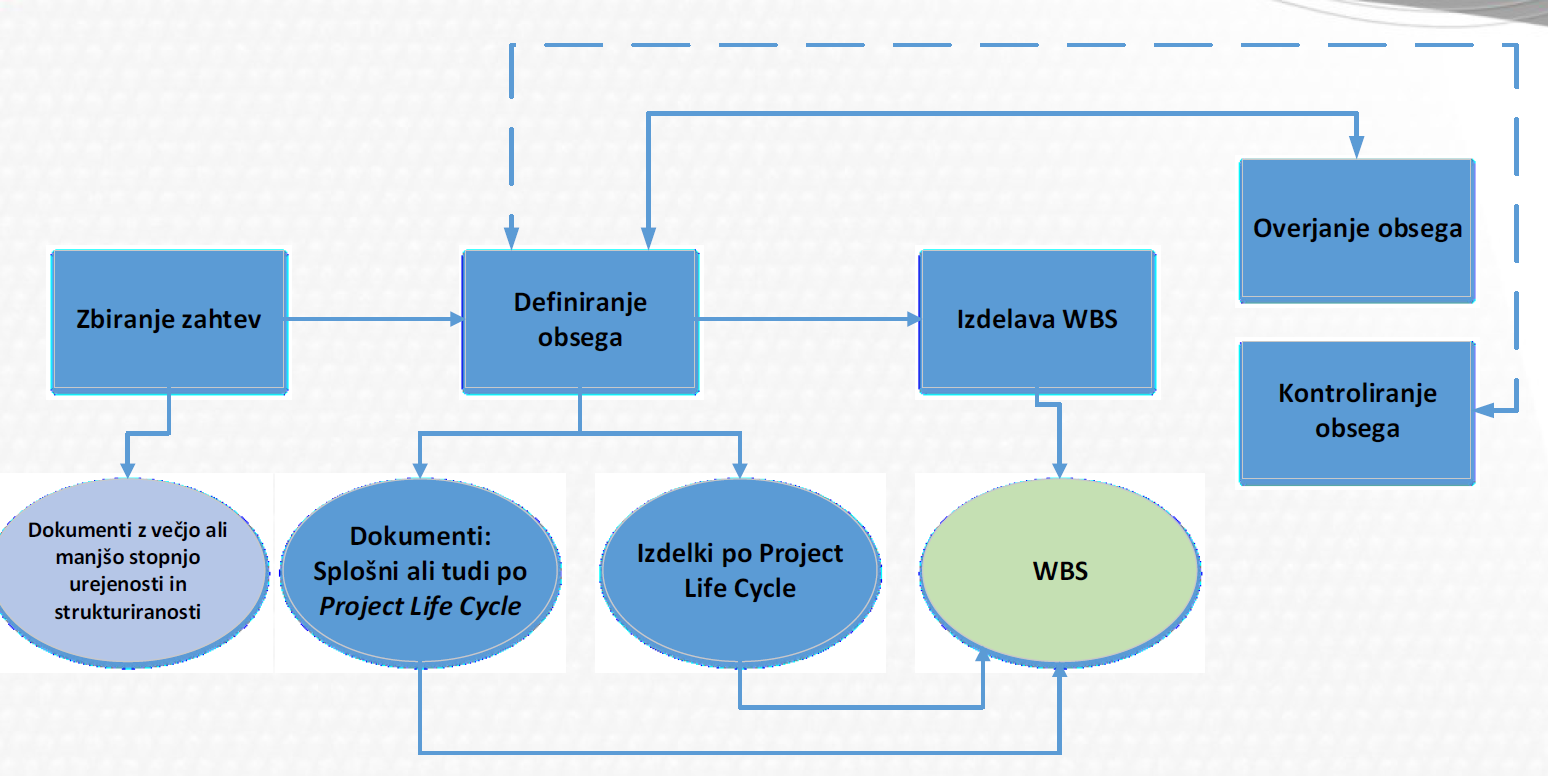
\includegraphics[scale=0.3]{011.png}

      \subsection{Definiranje obsega}
         \paragraph{Definiranje obsega} Opredeliti je potrebno kaj je in kaj ni obseg projekta, proces definiranja obsega je iterativen proces definiran s strani \emph{Project Life Cycle}.
         \paragraph{Overjanje obsega (z naročnikom)} V okviru procesa se sestajamo in usklajujemo obseg z naročnikom ter obseg formalno ali neformalno potrjujemo. Formalno preverjanje izvajamo vsaj ob mejnikih in na koncu projekta.
         \paragraph{Kontrola obsega (interno)} V definiranem obsegu nadziramo ali izdelki \emph{konvergirajo} v pravo smer. Pomembna je kontrola sprememb - spremembe obsega morajo biti definirane na podlagi odbritev, ne na podlagi \emph{telefonskih pogovorov} (formalne).


   \section{Obvladovanje časa}
      \begin{center}
         \begin{tabular}{|l|l|}
            \hline
            \textbf{Proces področja obvladovanja časa} & \textbf{Skupina procesov} \\
            \hline
            \hline
            Planiranje obvladovanja časa & Procesi planiranja \\
            Obvladovanje aktivnosti & \\
            Definiranje obsega & \\
            Razvrščanje aktivnosti & \\
            Ocenjevanje virov za aktivnost & \\
            Ocenjevanje trajanja aktivnosti & \\
            Pripravljanje terminskega plana & \\
            \hline
            Kontroliranje terminskega plana & Procesi nadzora in kontrole \\
            \hline
         \end{tabular}
      \end{center}
      
      \subsection{Opredeljevanje aktivnosti}
         \paragraph{}Opredelimo aktivnosti na delovne pakete. Aktivnosti so enote za katere je mogoče oceniti čas trajanja in katerih izvajanje je mogoče nadzirati. Aktivnosti razvrstimo in določimo njihov medsebojni vrstni red.
      \subsection{Ocenjevanje virov za aktivnosti}
         \paragraph{Človeški viri} Za aktivnost določimo izvajalec, lahko jih določimo poimensko, preko vlog ali, v primeru zunanjega izvajalca, preko imena podjetja. Pregled podatkov o zasedenosti virov je zahteven - saj zahteva pravo orodje in disciplino vnašanja ter posodabljanja podatkov.
         \paragraph{Ostali viri} Ostali viri aktivnosti so lahko oprema, ki je potrebna za aktivnost, material, \dots
      \subsection{Ocenjevanje trajanja aktivnosti}
         \paragraph{} Ocenjevanje trajanja aktivnosti ob upoštevanju določenih virov in obsega ter rezerv. Pri ocenjevanju trajanja si pomagamo iz baze znanja, posvetov ter izkušenj. Pripravimo lahko tudi več ocen za isto aktivnost \emph{pesimistično P, optimistično O in najbolj verjetno M}.
            \[ \frac{(P + 4M + O)}{6} \]
      \subsection{Priprava terminskega plana}
         \paragraph{Terminski plan} upošteva ocenjene čase trajanja in njihovo razvrstitev, dodatno še koledar (prazniki, vikendi, \dots).
         \paragraph{Kritična pot} Prikazuje pot na kateri so aktivnosti, katerih podaljšanje podaljša datum zakjučka projekta.
      \subsection{Kontroliranje terminskega plana}
         \paragraph{} Preverjamo kje smo v primerjavi s terminskim planom. Odstopanja predstavljajo zamujanje ali prehitevanje projekta - pri zamujah je potrebno poiskati faktorje zamujanja.
         \paragraph{Sestanki projektne ekipe za področje obvladovanja obsega in časa} Na sestankih se ugotavlja stanje izdelkov (napredek, ustreznost), odstopanja od terminskega plana (in razloge za odstopanja) ter spremembe terminskega plana ali obsega.
         \paragraph{Ključne naloge vodje projekta za področje obvladovanja obsega in časa} Obsegajo preverjanje izdelkov in trajanja aktivnosti z načrtom obsega in časa ter skrbi za komunikacijo med deležniki projekta.
   
   \section{Obvladovanje stroškov}
      \begin{center}
         \begin{tabular}{|l|l|}
            \hline
            \textbf{Proces področja obvladovanja stroškov} & \textbf{Skupina procesov} \\
            \hline
            \hline
            Planiranje obvladovanja stroškov & Procesi planiranja \\
            Ocenjevanje stroškov & \\
            Določanje proračuna & \\
            \hline
            Nadzor stroškov & Procesi nadzora in kontrole \\
            \hline
         \end{tabular}
      \end{center}

      \subsection{Ocenjevanje stroškov}
         \paragraph{Vrste stroškov}
            \begin{itemize}
               \item fiksni stroški in variabilni stroški
               \item stroški dela, materiala in opreme
               \item stroški licenc
               \item stroški dela podizvajalcev
            \end{itemize}
         \paragraph{Metodologija ocenjevanja stroškov} je odvisna od podjetja in določi katere vrste stroškov se v okviru planiranja ocenjuje.
      
      \subsection{Določanje proračuna}
         \paragraph{} Proračun se določa z agregiranjem vseh stroškov od spodaj navzgor, pri čemer se določi tudi rezervo, s katero razpolaga vodja projekta samostojno, in rezervo, katero odobri projektni svet.
      \subsection{Nadzor stroškov}
         \paragraph{} Nadzor se izvaja na posamezni aktivnosti in na projektu kot celota. Nadzira se tiste stroške, ki jih ocenjujemo in za njih sproti vnašamo porabo. Nadzor in pravila so določena na nivoju podjetja.

   \section{Obvladovanje kakovosti}
      \paragraph{Kaj je kakovost?} Kakovost delimo na kakovost končnega izdelka in kakovost procesa s katerim izdelujemo končni izdelek. Po PMBoK je trab obvladovati kakovost, same pristope in tehnike pa določa project life cycle. Pri projektih razvoja je kakovost določena s testiranjem.
      \begin{center}
         \begin{tabular}{|l|l|}
            \hline
            \textbf{Proces področja obvladovanja časa} & \textbf{Skupina procesov} \\
            \hline
            \hline
            Planiranje kakovosti & Procesi planiranja \\
            \hline
            Izvajanje zagotavljanja kakovosti & Procesi izvajanja \\
            \hline
            Izvajanja nadzora kakovosti & Procesi nadzora in kontrole \\
            \hline
         \end{tabular}
      \end{center}
   
      \subsection{Planiranje kakovosti}
         \paragraph{Postavitev zahtev} Osnova zahtev glede kakovosti so praviloma standardi in standardne matrike. Osnove lahko postavimo že v VDP. Naročnik lahko postavi posebne zahteve glede kakovosti (predvsem pri kritičnih sistemih).
         \paragraph{Tipični koncepti testiranja}
            \begin{itemize}
               \item planiranje \emph{enot} testiranja: unit testi, testi modulov, testi celote, testi integracij,\dots
               \item testiranje migracij podatkov
               \item potrditveni test
            \end{itemize}

      \subsection{Izvajanje zagotavljanja kakovosti}
         \paragraph{Standardi} V primeru razvoja programske opreme pod to štejemo uporabo dobrih praks in internih standardov.
         \paragraph{Metodologija} V primeru razvoja programske opreme gre za uporabo interne metodologije razvoja programske opreme.
         \paragraph{V splošnem} Gre za standardne procese, ki upoštevajo najboljše prakse in interne izkušnje, ki z visoko verjetnostjo zagotavljajo kakovosten izdelek.

      \subsection{Izvajanje nadzora in kontrole}
         \paragraph{Izvajanje testiranj in zagotavljanje sledljivosti} POtrebno je beležiti vse teste, njihove rezultate ter uagotoviti sledljivost ponovnega testiranja napak in zabeležitve statusa odprav napak.

   \section{Obvladovanje človeških virov}
      \begin{center}
         \begin{tabular}{|l|l|}
            \hline
            \textbf{Proces področja obvladovanja časa} & \textbf{Skupina procesov} \\
            \hline
            \hline
            Planiranje človeških virov & Procesi planiranja \\
            \hline
            Pridobivanje projektne ekipe & Procesi izvajanja \\
            Razvoj projektne ekipe & \\
            Obvladovanje projektne ekipe & \\
            \hline
         \end{tabular}
      \end{center}

      \subsection{Planiranje človeških virov}
         \paragraph{} PLanirati je potrebno člane projektne ekipe, njivoe vloge, glavne naloge in odgovornosti ter nagrajevanja glede na uspešnost. Osnovo predstavlja VDP.
         \paragraph{} Določi se stališča glede zapolnjevanja vrzeli (nove zaposlitve) ter način sodelovanja s podpornimi službami (kadrovska služba, nabava,\dots).
      \subsection{Pridobivanje projektne ekipe}
         \paragraph{} V primeru manjših projektov je ta proces povezan s planiranjem, v splošnem pa proces vključuje pridobivanje novih kadrov in pogajanja za interne kadre.
      \subsection{Razvoj projektne ekipe}
         \paragraph{} Vključuje team buildinge, spodbujanje članov, njihovo izobraževanje ter postavljanje pravil (zamujanje na sestanke, etika, komunikacija,\dots).
      \subsection{Obvladovanje projektne ekipe}
         \paragraph{} Vodja projekta skrbi za delovanje celotne ekipe in dleovanje posameznikov znotraj ekipe, skrbi za komunikacijo in razreševanje konfliktov med člani projektne ekipe.

   \section{Obvladovanje komuniciranja na projektu}
      \begin{center}
         \begin{tabular}{|l|l|}
            \hline
            \textbf{Proces področja obvladovanja komuniciranja} & \textbf{Skupina procesov} \\
            \hline
            \hline
            Planiranje obvladovanja komuniciranja & Procesi planiranja \\
            \hline
            Izvajanje komuniciranja & Procesi izvajanja \\
            \hline
            Nadzor komuniciranja &  Procesi nadzora in kontrole \\
            \hline
         \end{tabular}
      \end{center}

      \subsection{Izvajanje komuniciranja}
         \paragraph{} Komuniciranje vključuje kreiranje, zbiranje, shranjevanje in distribuiranje podatkov ter informacij o projektu. Mediji komuniciranja vsebujejo pisno komuniciranje, elektronsko pošto, telefonske pogovore, sestanke, \dots
         \paragraph{Posredovanje ciljni skupini} Vsaka ciljna skupina deležnikov mora dobiti sebi primerno informacijo.
         \paragraph{Formalno poročanje} (statusno poročilo) je del komuniciranja.
      \subsection{Sestanki}
         \paragraph{Planiranje} Sestnke je potrebno planirati v naprej (predvsem ponavljajoče sestanke za daljše obdobje), njihovo dolžino in vsebino, ki se je je potrebno držati. Sestanek naj ima dnevni red in cilj, ki ga udeleženci poznajo v naprej.
         \paragraph{Količina sestankov} Sestankov ne sme biti preveč, prepogosto in ne smejo biti predolgi. Vsak sestanek naj oloči naloge, cilje in časovne roke. Za vsak sestanek naj se pripravi zapisnik.
      \subsection{Nadzor komuniciranja}
         \paragraph{} Stalen nadzor nad prejemom in oddajo informacij vsaki izmed ciljnih skupin. Ciljna skupina mora prejeti sebi primerne informacije ter jih pravilno razumeti.
      \subsection{Poročanje}
         \paragraph{Poročila in frekvence poročanja} VDP že v naprej doreče tipe in frekvence poročil, ne določa pa podrobnosti poročila. V poročila vključimo primerjavo med planom in trenutnim stanjem ter \emph{pogled v naprej}. Poročila naj bodo jedrnata, brez prikrivanja dejstev in problemov.

   \section{Obvladovanje tveganj na projektu}
      \begin{center}
         \begin{tabular}{|l|l|}
            \hline
            \textbf{Proces področja obvladovanja tveganj} & \textbf{Skupina procesov} \\
            \hline
            \hline
            Planiranje obvladovanja tveganj & Procesi planiranja \\
            Identifikacija tveganj & \\
            Izvajanje kvalitativne analize tveganj & \\
            Izvajanje kvantitativne analize tveganj & \\
            Planiranje odzivov na nastop tveganj & \\
            \hline
            Nadziranje tveganj & Procesi nadzora in kontrole \\
            \hline
         \end{tabular}
      \end{center}

      \subsection{PLaniranje obvladovanja tveganj}
         \paragraph{Osnovni koncepti obvladovanja tveganj} Osnovni koncepti vsebujejo pristope in orodja, vloge in odgovornosti, časovne okvirje, definicije za verjetnost in vpliv, amtrike verjetnost - vpliv, \dots
         \paragraph{Plan obvladovanja tveganj} Plan zagotavlja lažji prevzem vodenja projekta s strani novega projektne vodje. Odločitev ali se takšen plan izdela ali ne, pa je interna odločitev podjetja.

      \subsection{Identifikacija tveganj}
         \paragraph{Identifikacija} se izvede na podlagi izkušenj in baze znanja. Izvaja jo projektna ekipa, sponzor, ostali deležniki in po potrebi zunanji svetovalci, pri čemer imajo podobni projekti podobna tveganja.
         \paragraph{Skrbnik tveganj} je oseba, ki je odgovoren za kritična tvganja projekta.
         \paragraph{Statusi tveganj} odprt (v obravnavi), zaprt, ponovno odprt.

      \subsection{Kvalitativna in kvantitativna analiza tveganj}
         \paragraph{Kvalitativna analiza tveganj} dodatno opisuje identificirana tveganja, določa verjetnost posameznim tveganjem ter njihov vpliv. V VDP podamo tveganja skupaj z verjetnostmi in vplivom.
         \paragraph{Kvantitativna analiza tveganj} finančno ovrednoti tveganje - koliko nas bo stalo, če se tveganje uresniči. Cilj kvantitativne analize je zavarovanje tveganj.

      \subsection{Planiranje odzivov na nastop tveganj}
         \paragraph{} Odzive planiramo za kritična tveganja, osnovo za odziv pa postavimo že v VDP.
         \paragraph{Skrbnik tveganja} je odgovore za dva kjučna elementa:
            \begin{itemize}
               \item opredelitev potrebne aktivnosti in odgovornosti, ko se tveganje zgodi
               \item opredelitev potrebne aktivnosti in odgovornosti, ki z visoko stopnjo verjetnosti preprečijo tveganje
            \end{itemize}
         \paragraph{Posledica in rezultat procesa} so lahko spremembe v obsegu projekta, terminkem planu, planu kakovosti, oskrbovanja, človeških virov in/ali stroškov.
      
      \subsection{Nadziranje tveganj}
         \paragraph{} Vključuje spremljanje identificiranih tveganj ter odkrivanje novih, spreminjanje ocene verjetnosti in/ali vpliva, zapiranje tveganj ter zatevek za spremembo za preprečevanje tveganja.

   \section{Obvladovanje oskrbovanja na projektu}
      \begin{center}
         \begin{tabular}{|l|l|}
            \hline
            \textbf{Proces področja obvladovanja oskrbovanja} & \textbf{Skupina procesov} \\
            \hline
            \hline
            Planiranje oskrbovanja & Procesi planiranja \\
            \hline
            Izvajanje oskrbovanja & Procesi izvajanja \\
            \hline
            Administracija oskrbovanja & Procesi nadzora in kontrole \\
            \hline
            Zapiranje pogodb & Procesi zapiranja \\
            \hline
         \end{tabular}
      \end{center}

      \subsection{Planiranje oskrbovanja}
         \paragraph{Analiza naredi ali kupi} Pri analizi je potrebno določiti obseg za vsako izemd zunanjih izvajanj, materiala in opreme za nabavo, določiti tipe pogodb (fixed price, time and material).
      \subsection{Izvajanje oskrbovanja}
         \paragraph{} Pri tem procesu aktivno sodeluje nabavna služba in vključuje povabila k oddaji ponudb, pogajanja, izbor zunanjih izvajalcev in dobaviteljev ter podpisovanje pogodb.
      \subsection{Administracija oskrbovanja}
         \paragraph{} Gre za obvladovanje pogodbenih razmerij z zunanjimi izvajalci in dobavitelji, nadzor poročanja s strani zunanjih izvajalcev, preverjanje in potrjevanje prejetih računov ter prekinjanje pogodb.
         \paragraph{Aneksi k pogodbam} vse spremembe pogodb na projektu običajno potrjuje projektni vodja ali projektni svet.
      \subsection{Zapiranje pogodb}
         \paragraph{} Potrebno je podrobno preverjanje izpolnjevanja obveznosti, podpis prevzemnega zapisnika za dobavitelje in zunanje izvajalce ter potrditev in plačilo končnega računa.

   \section{Obvladovanje pričakovanj deležnikov}
      \begin{center}
         \begin{tabular}{|l|l|}
            \hline
            \textbf{Proces področja obvladovanja pričakovanj} & \textbf{Skupina procesov} \\
            \hline
            \hline
            Identifikacija deležnikov & Procesi inicializacije \\
            \hline
            Planiranje obvladovanja deežnikov & Procesi planiranja \\
            \hline
            Obvladovanje pričakovanj in sodelovanja deležnikov & Procesi izvajanja \\
            \hline
            Nadzor pričakovanj in sodelovanja deležnikov & Procesi nadzora in kontrole \\
            \hline
         \end{tabular}
      \end{center}

      \subsection{Identifikacija deležnikov}
         \paragraph{Odkrivanje deležnikov} Pridobiti je potrebno informacije o vseh deležnikih na projektu, o njihovem vplivu, sponzorstvu in naklonjenosti.
         \paragraph{Register deležnikov} je tajen dokument z vsemi podatki o posameznih deležnikihm njihovi klasifikaciji (podpornik, nevtrale, nasprotnik), beleženjem opazk in načinom komuniciranja.
      \subsection{Obvladovanje pričakovanj in sodelovanja deležnikov}
         \paragraph{Stabilnost projekta} Deležniki pogosto želijo spremeniti obseg projekta (nove zahteve, spremembe zahtev), zato je glavni cilj povečati podporo projektu s strani ključnih deležnikov, ki imajo vpliv na projekt.
      \subsection{Nadzor pričakovanj in sodelovanja deležnikov}
         \paragraph{Nadzor do in med deležniki} Spremljanje morebitnih sprememb v vplivu, položaju in moči posameznih deležnikov v projektu. Po potrebi se plan obvladovanja deležnikov spreminja.

   \section{Integracija projekta}
      \paragraph{Procesi integracije projekta}
         \begin{itemize}
            \item izdelava VDP
            \item izdelava projektnega plana
            \item usmerjanje in vodenje izvajanja projekta
            \item opazovanje in nadziranje projektnega dela
            \item izvajanje integriranega nadzora potrebnih sprememb
            \item zapiranje projekta ali faze
         \end{itemize}

      \subsection{Izdelava VDP}
         \paragraph{VDP} Dokument s katerim naročnik in izvajalec potrdita cilje, vsebino in ostale elemente projekta ter vzpostavita partnerstvo, Sktruktura VDP je lahko eneka strukturi ponudbe, z razliko, da VDP nima sklopa o ceni oz. vrednosti.
         \paragraph{Struktura VDP} VDP naj vsebuje povzetek za vodstvo (jedrnatom, ne preveč ITjevsko), jasne in merljive cilje projekta ter pričakovane koristi projekta, ki naj bodo razumljive poslovnim uporabnikom. VDP naj vsebuje tudi tehnične izdelke (vmesne in končne izdelke s prevzemnimi kriteriji), projektne izdelke (VDP, plan upravljanja s tveganje, prevzemne zapisnike,\dots), opredelitev izdelkov, rezultatov in učinkov, ki jih projekt ne bo dal ter predpostavke, omejitve in predpogoje za uspešen zaključek projekta. Na konc se v VDP vključi organizacijsko strukturo, koordinacijo z morebitnimi drugimi projekti ter tveganja.
         \paragraph{Terminski plan in ključni mejniki} VDP naj vsebuje tudi WBS na zelo visokem nivoju ter gentogram skupaj z mejniki, ki definirajo kdaj in kaj se ob mejniku zgodi (predaja izdelka).
      
      \subsection{Izdelava projektnega plana}
         \paragraph{Projektni plan} ni identičen terminskemu planu, projektni plan vključuje plan vodenja projekta in definira kako se projekt planira, izvaja, nadzira in zapre. Gre za koordinacijo izdelave planov na področju znanja in združitev vseh planov (obvladovanje obsega, časa, kakovosti,\dots).
      \subsection{Usmerjanje in vodenje izvajanja projekta}
         \paragraph{Usmerjanje glede}
            \begin{itemize}
               \item na projektni plan
               \item odobrene zahteve za spremembe
               \item poznavanje project life cycle
               \item na podlagi: korektivnih in preventivnih ukrepov ter odpravljanje škode
            \end{itemize}
      \subsection{Obvladovanje znanj projekta}
         \begin{itemize}
            \item polnjenje baze
            \item eksplicitno znanje in tacitno znanje
            \item vzpostavitev atmosfere, v kateri člani delijo znanje in izkušnje
         \end{itemize}

      \subsection{Opazovanje in nadziranje projektnega dela}
         \paragraph{Zbiranje podatkov} za spremljanje poteka projekta, izdelavo statusni poročil in izdelavo napovedi.
         \paragraph{Rezultat opazovanja} je lahko del vhodnih podatkov za pripravo načrta tveganj in zahtvekov za spremembo.

      \subsection{Izvajanje integriranega nadzora potrebnih sprememb}
         \paragraph{Ključen proces} Omogoča pregled zatevkov za spremembo na (praviloma) obsegu, časovnih terminih in cenovnih komponentah sistema. Interne spremembe lahko potrjuje vodja projekta sam, druge potrjuje naročnik ali projektni svet.
      \subsection{Zapiranje projekta ali faze}
         \paragraph{Predaja izdelkov} Vključuje predajo izdelkov, potrditev prevzema (s prevzemnim zapisnikom) in interno obogatitvijo baze znanja za prihodnje projekte.
   
\end{document}